\chapter{The First Analog Prototype}~\label{chap:saq}

In this chapter we present the first implementation of the Q-Pix front-end design using off-the-shelf electronics.

This section describes the first prototype based on the Q-Pix readout: The Simplified Analog Q-Pix (SAQ).
First we discuss the design goals of the prototype and highlight the basic building blocks of any Q-Pix based prototype.
We present these results as a demonstration Q-Pix timestamp procedure to perform measurements.
Next, we describe the prototype status as well as lessons learned in characterizing noise and performing calibrations.

In the final part of this section we briefly describe the future goals of this prototype, including the calibration of the detector response with Gas Electron Multipliers (GEMs)~\citep{SAULI20162}.
We emphasize that at the time of the writing of this thesis the acquisition and analysis of data from this experiment are incomplete.
Nevertheless, the lessons learned so far, particularly in calibration, are useful to explore the abilities of the Q-Pix readout.
The final results of SAQ are just beyond the scope of this work, but we provide SAQ's details here as a means of introducing the front-end of Q-Pix as well as highlighting my personal contributions to Q-Pix's overall development.

The entire data acquisition (DAQ) chain used for both SAQ experimental setups are my sole independent work.
My contributions include the the development and deployment firmware on the Zybo-Z7 FPGA, as well as the embedded software code on the integrated SoC processing system.
I developed the the Python3 software which handles packet communication as well as the GUI for data collection.
I also developed the data storage trees, which are the original containers for all data used in the analysis. 
Additionally, I wrote analysis scripts used for the work done at the SAQ site at the University of Texas at Arlington.

\section{Simplified Analog Q-Pix: System Design}
The Simplified Analog Q-Pix (SAQ) experiment aims to demonstrate the first physics measurement using the analog front-end of a Q-Pix based readout.
The desired measurement is the transverse diffusion of electron in Argon gas~(Equation~\ref{eq:diffusion}).
In the simplest case, the diffusion of electrons within a TPC is described by:
\begin{equation}~\label{eq:diffusion}
 \sigma^{2}_{T} = 2D_{\mathrm{trans}}L
\end{equation}
Where L is the drift length of the electrons, $D_{\mathrm{trans}}$ is the (field dependent) diffusion coefficient, and $\sigma_{T}$ is the transverse diffusion standard deviation.
A Q-Pix readout could perform a measurement of $D_{\mathrm{trans}}$ in Equation~\ref{eq:diffusion} by collecting charge at different radii from the center.

Measurements of transverse and longitudinal diffusion of electrons within electric fields of strength 50~\unit{\frac{V}{cm}} have been performed before~\citep{lar_diffusion_measurement_LI2016160}.
A diffusion measurement is a natural starting point to verify a charge accumulation readout such as Q-Pix.
One difference between SAQ and a "normal" Q-Pix readout is that instead of an array of pixels, SAQ uses a series of 16 concentric rings to collect charge.
Although a 2-D array of pixels may be used, since transverse diffusion is radially symmetric about the collection plane rings of different radii will collect different amounts of charge according to Equation~\ref{eq:diffusion}
Also, the use of circular 'pixels' reduces the amount digitization channels in the prototype.

SAQ has built two different TPCs: one at the University of Texas at Arlington (UTA) and the other at Wellesley College (WC).
The experimental setup at UTA is shown in Figure~\ref{fig:saq_setup_flatten}, and the setup at Wellesley is shown in Figure~\ref{fig:wellesley_tpc}.
Both TPCs shown are circular TPCs with a drift length of $\approx 10~\unit{cm}$.

The experimental setups at both UTA and Wellesley are nearly identical except for the placement of the readout electronics.
The SAQ readout board for UTA is placed on the outside of the TPC, whereas at WC it is placed within a P10 argon gas, but not within the field cage of the TPC.
The drift medium used within the TPC at UTA is an ultra pure (99.99\%) argon gas.

\begin{figure}[]
\centering
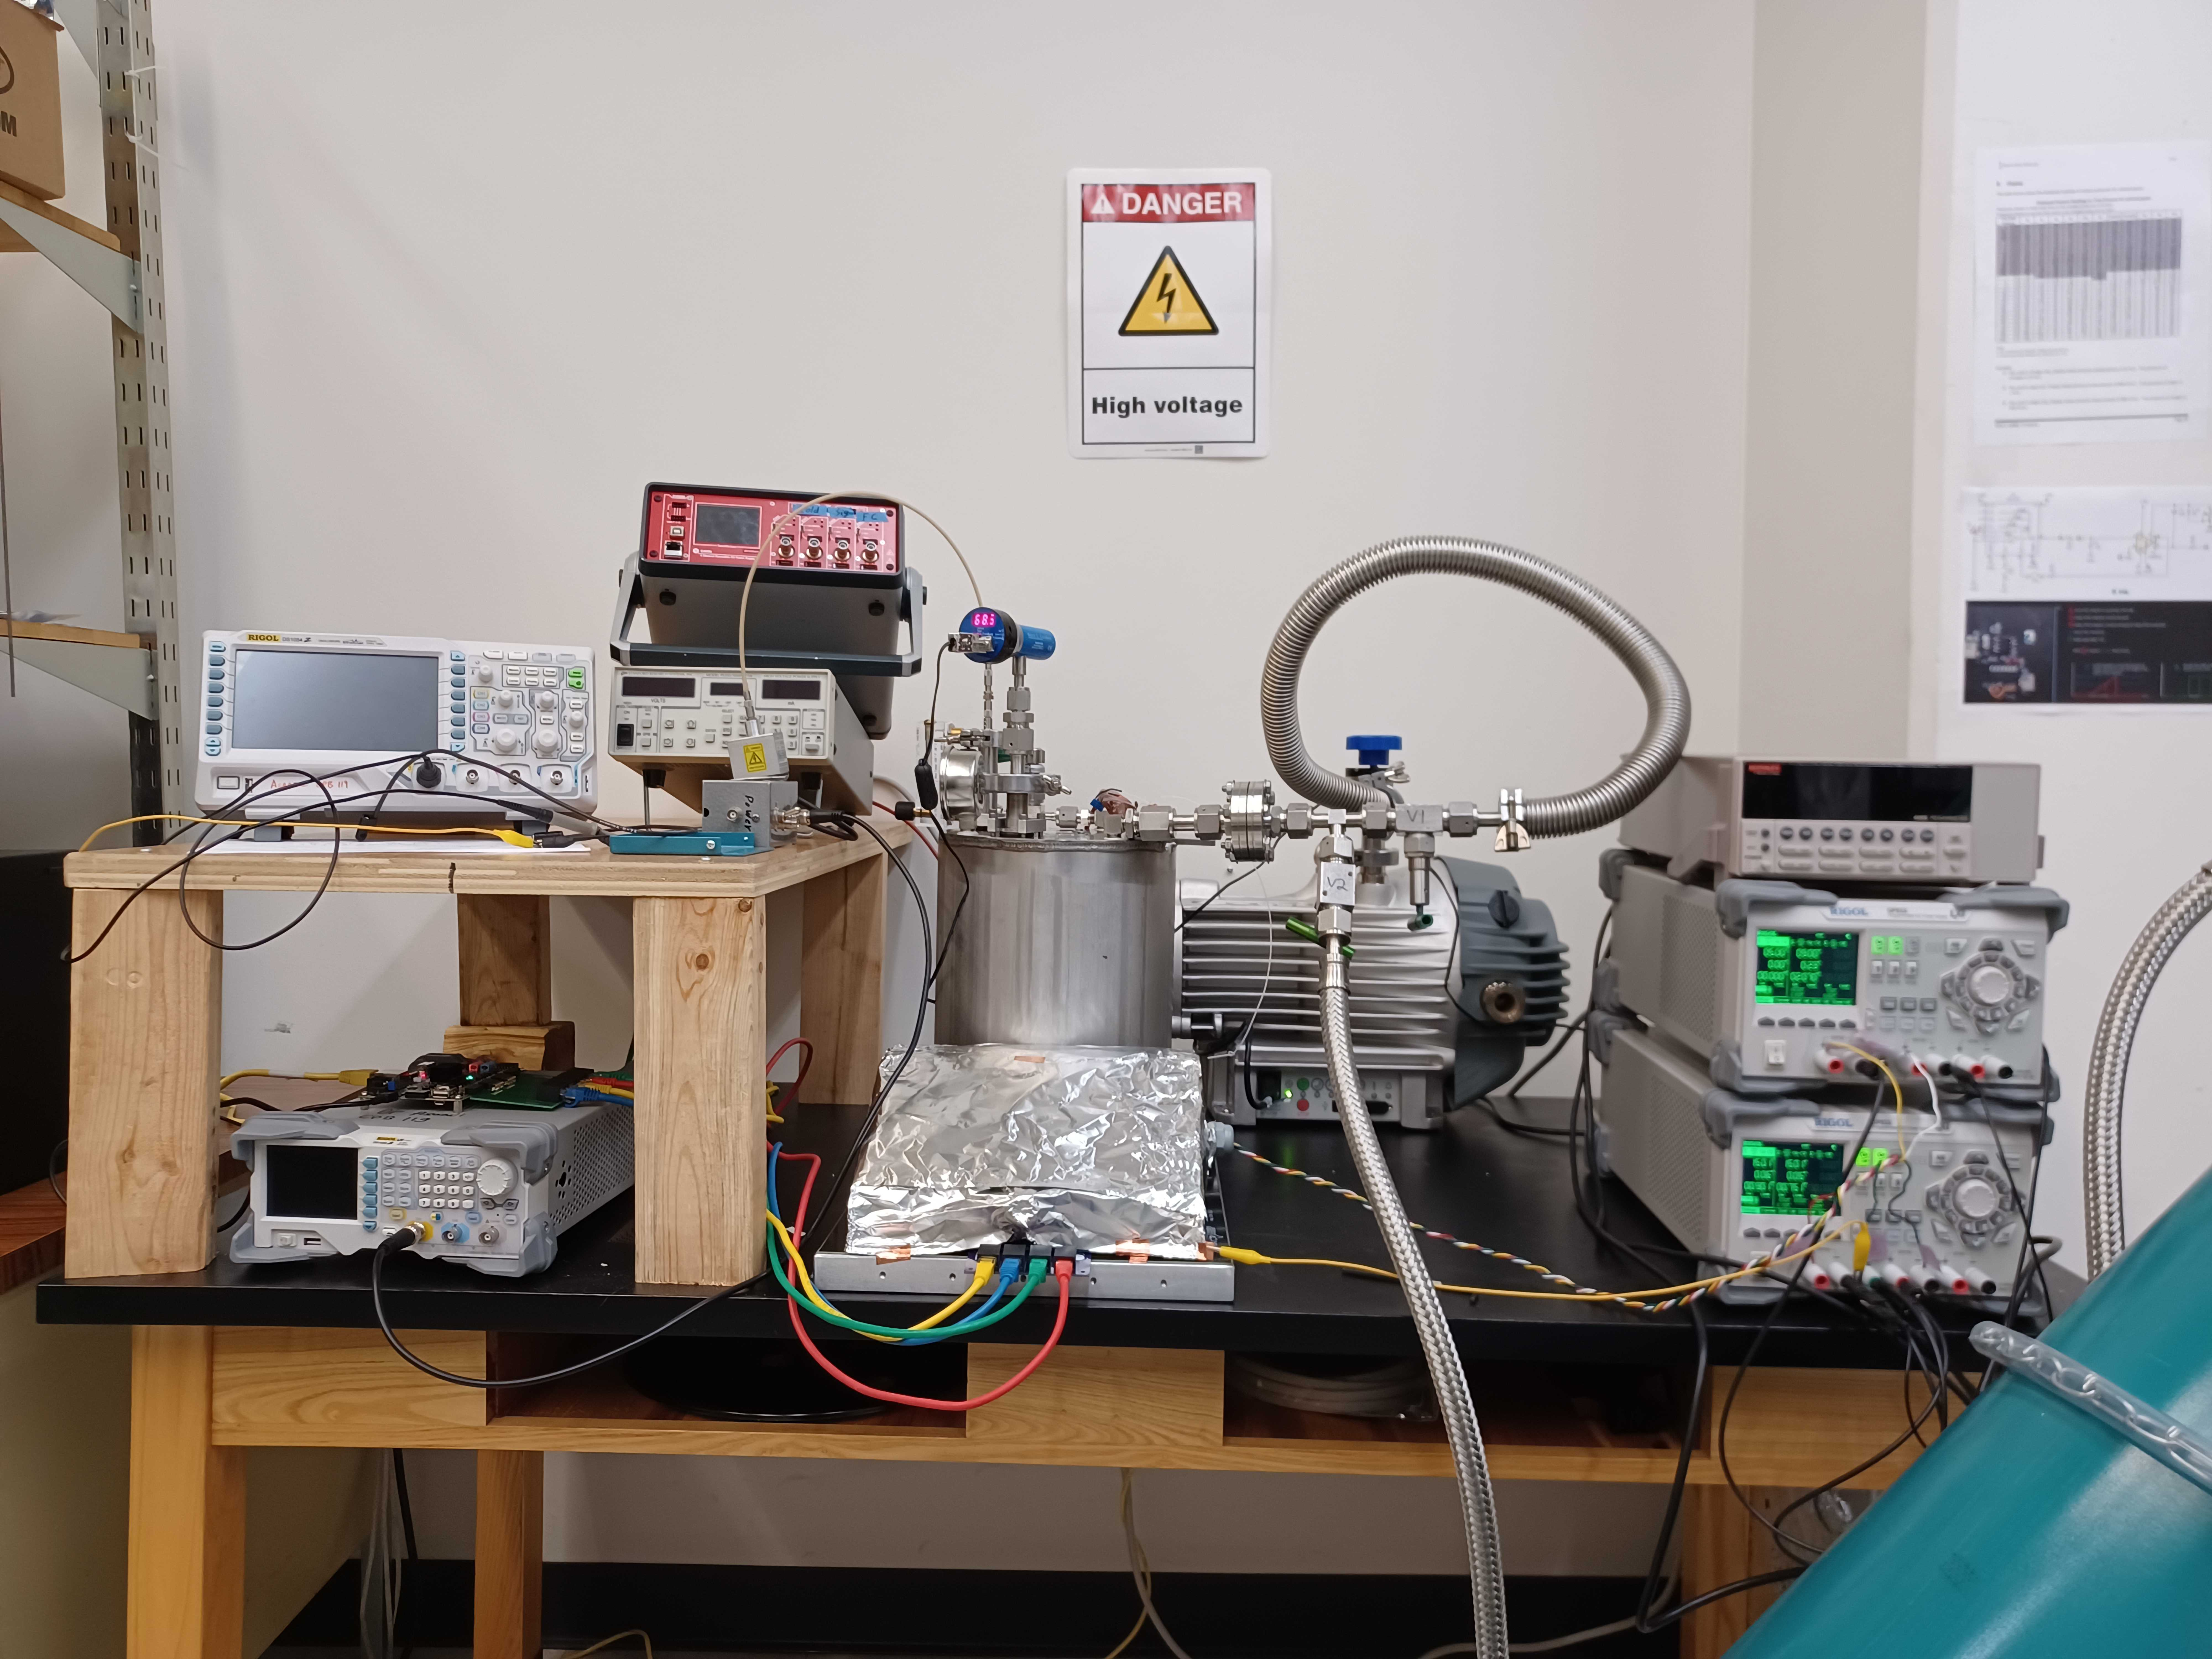
\includegraphics[width=\textwidth]{images/SAQ_physical_setup.jpg}
\caption{The SAQ setup at UTA.
In the center is the TPC, SAQ board~(Figure~\ref{fig:saq_readout_board}), and pump as shown in Figure~\ref{fig:saq_physical_setup_flatten}.
}
\label{fig:saq_setup_flatten}
\end{figure}

\begin{figure}[]
\centering
\begin{subfigure}{.5\textwidth}
  \centering
  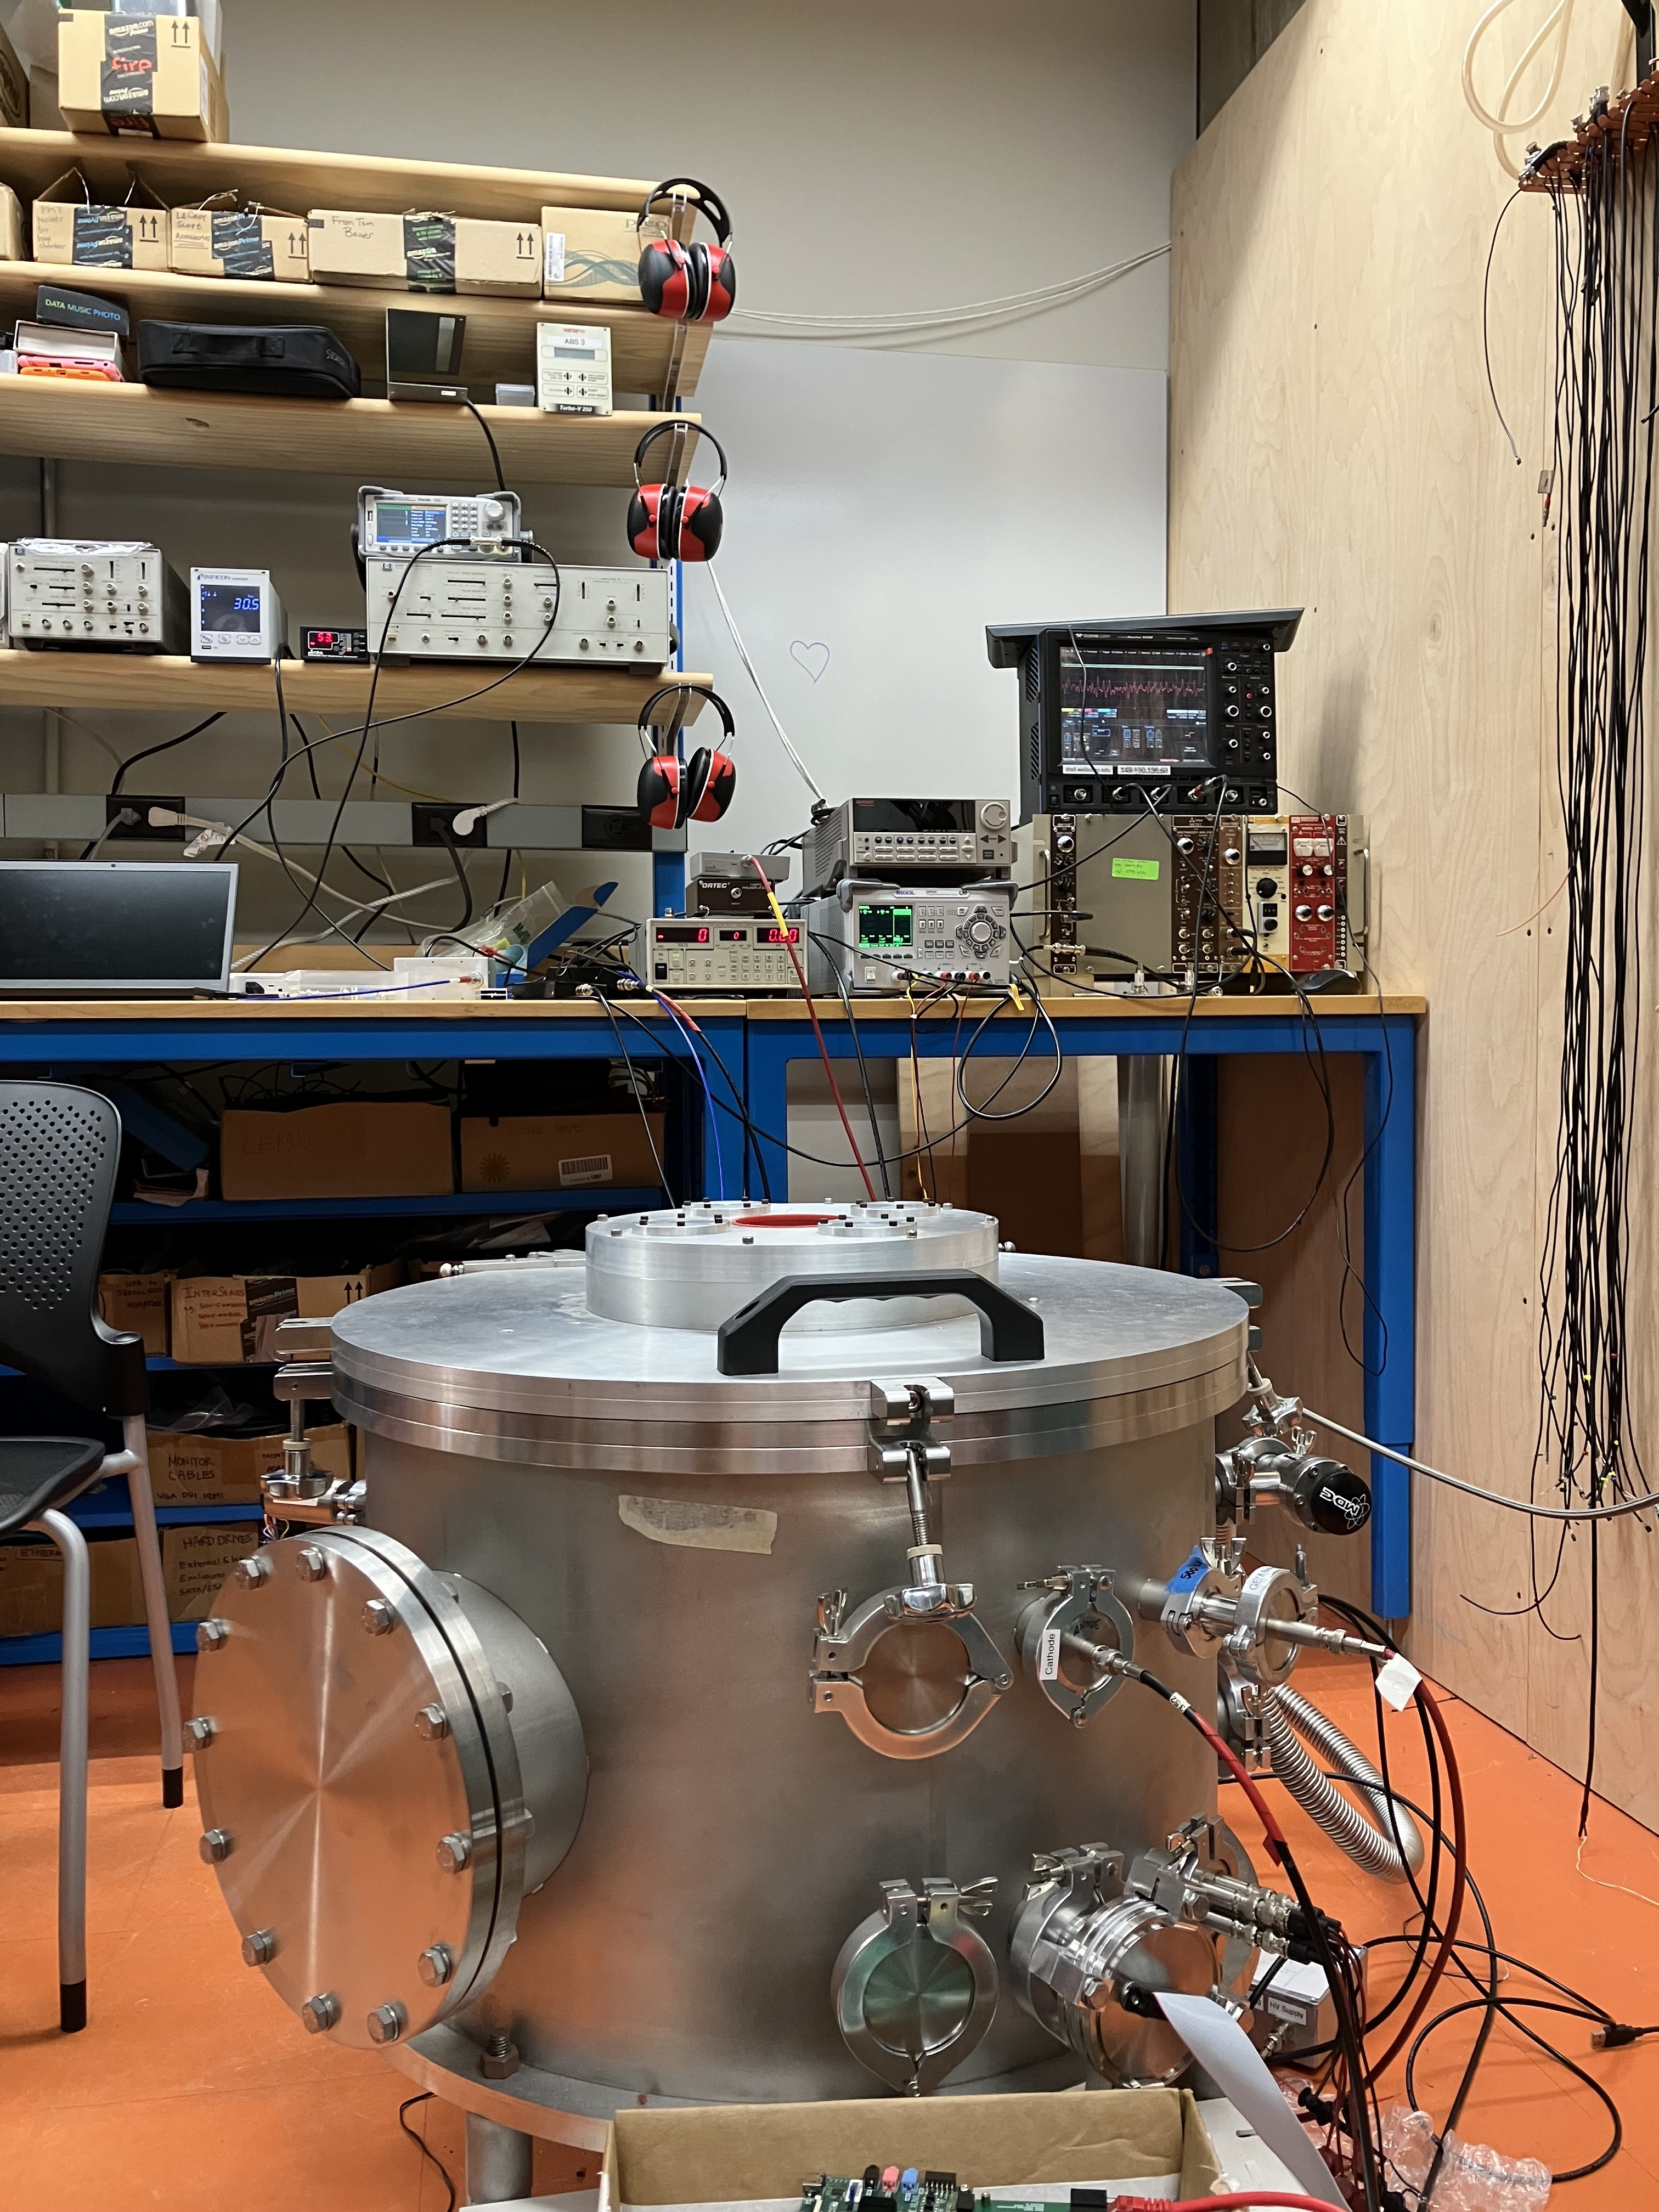
\includegraphics[width=\textwidth]{images/saq_wellesley_tpc.jpg}
  \caption{}
\end{subfigure}%
\begin{subfigure}{.5\textwidth}
  \centering
  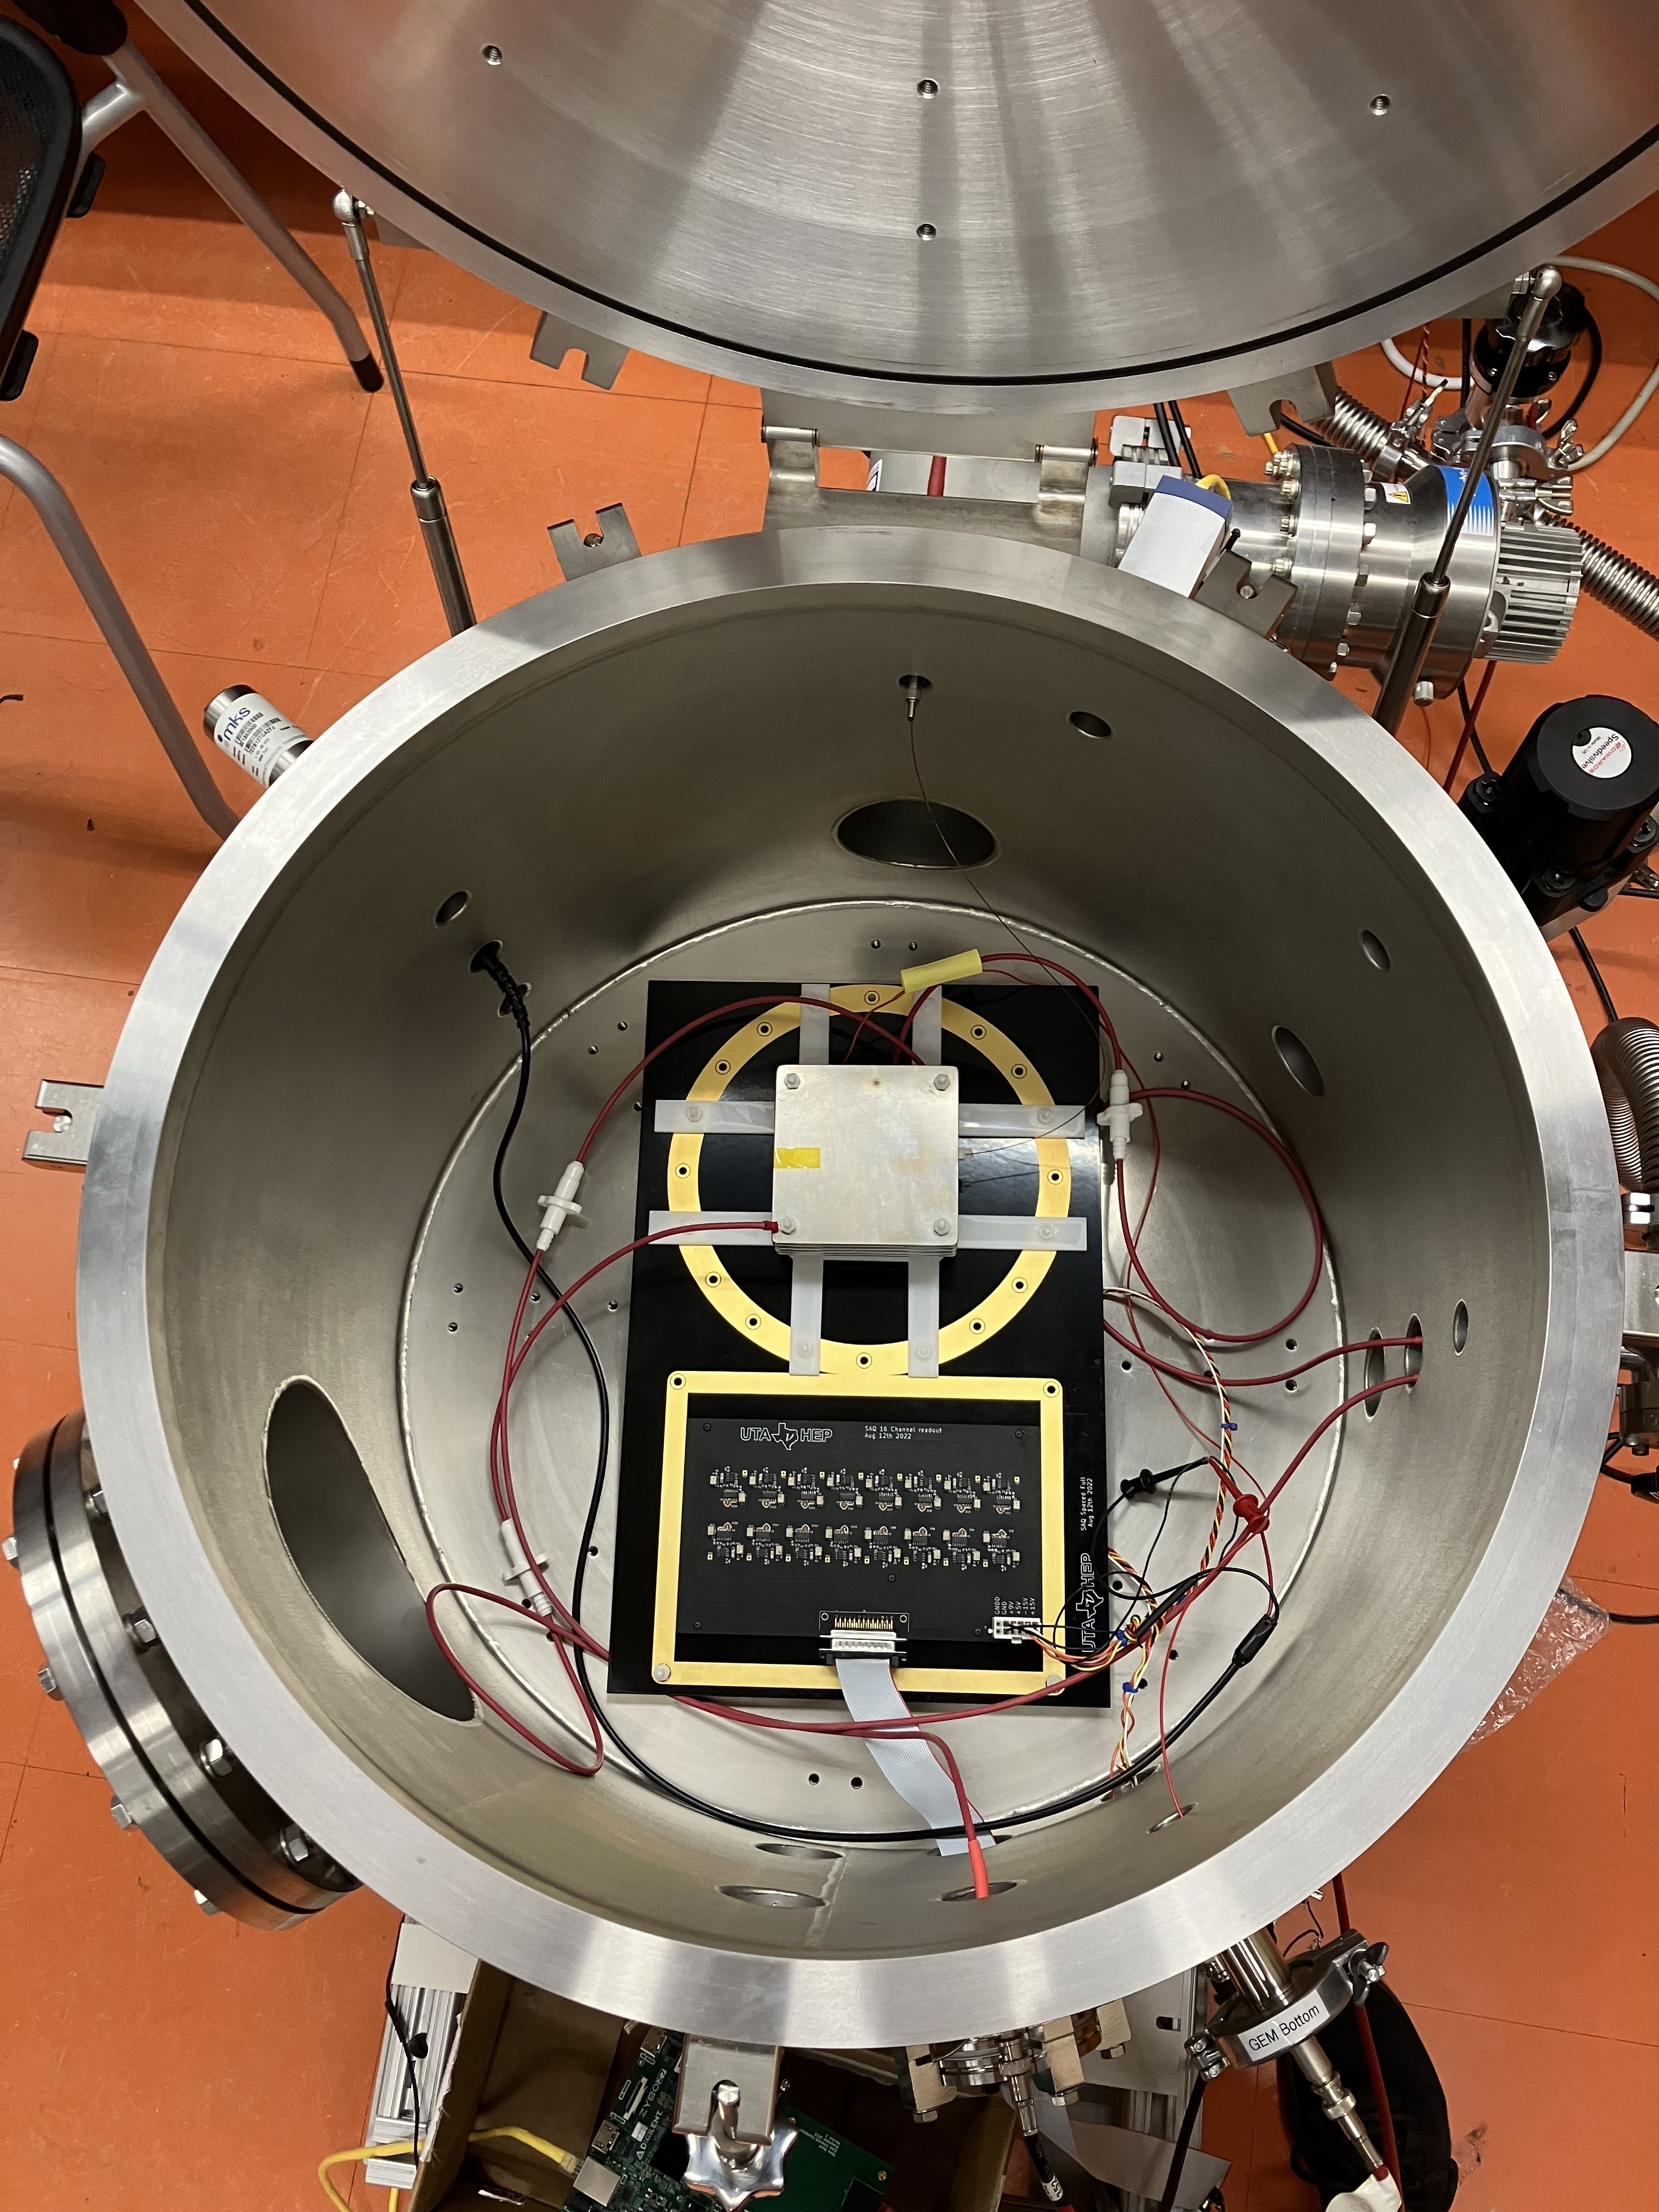
\includegraphics[width=\textwidth]{images/saq_wellesley_tpc_daq.jpg}
  \caption{}
\end{subfigure}
\caption{Picture of the TPC and DAQ setups at Wellesley University.
Image of the TPC cage (left) is used to store P-10 Argon gas. P-10 Argon gas uses a 10\% mixture of methane, and prevents sparking from the high-voltage of the TPC.
Inside of the TPC (right) shows the SAQ readout board.
The SAQ readout board is used at both UTA and Wellesley.
}
\label{fig:wellesley_tpc}
\end{figure}

Electrons are produced in the TPC from gold foil and a Hamamatsu L13651~\citep{hamamatsu_tls1023e} Xenon Gas Lamp via the photo-electric effect~\citep{https://doi.org/10.1002/andp.19053220607}.
As the electrons are removed from the gold, they enter the electric field and are drifted down to a collection plane.
A simplified image of the working TPC, rings, and GEM placement are shown in Figure~\ref{fig:saq_physical_setup_flatten}.
The design of the GEM PCB as well as its operating voltages is based on work presented in~\citep{THORPE2023167438}.
The GEM is used to provide a necessary charge amplification ($\sim 10^{3}$) per channel to induce resets in rings far from the center.

\begin{figure}[]
\centering
\begin{subfigure}{.45\textwidth}
  \centering
  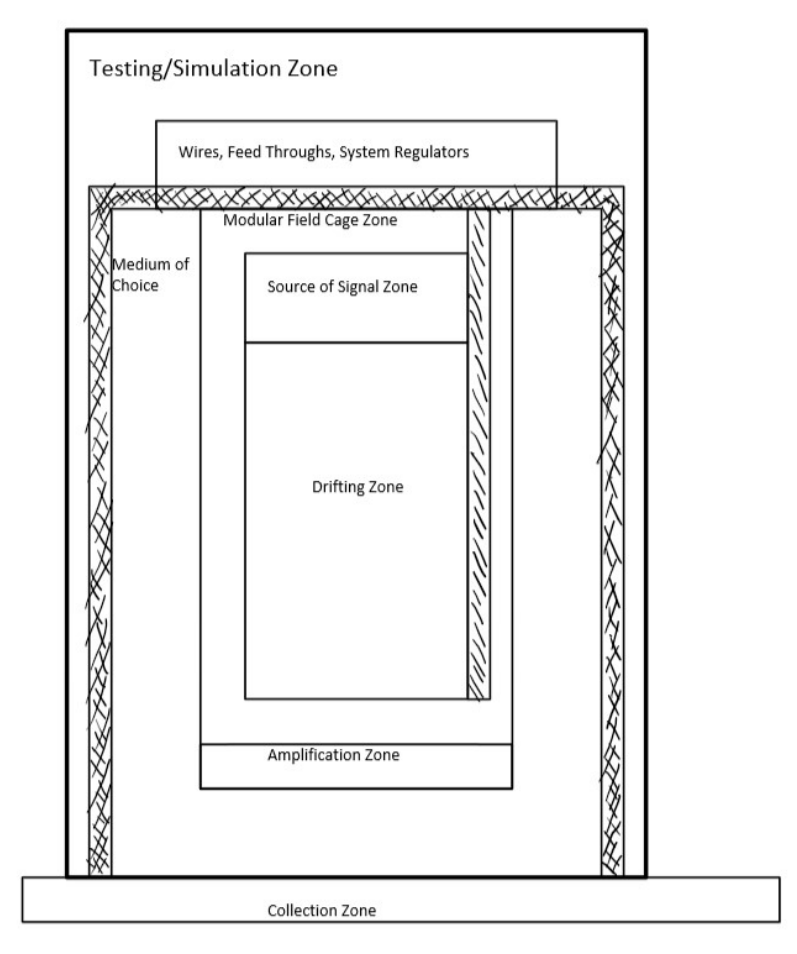
\includegraphics[width=\textwidth]{images/saq_tpc_insides.png}
  \caption{}
\end{subfigure}%
\begin{subfigure}{.38\textwidth}
  \centering
  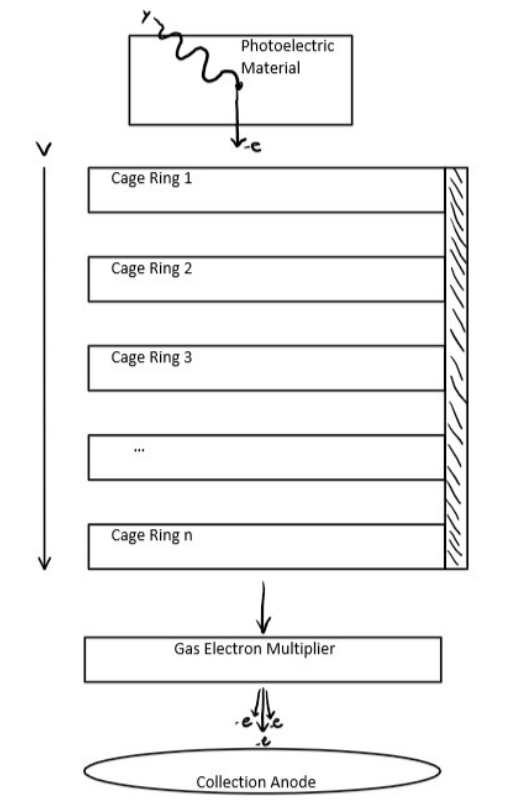
\includegraphics[width=\textwidth]{images/saq_rings_insides.png}
  \caption{}
\end{subfigure}
\caption{The SAQ model shown explicitly Figure~\ref{fig:saq_setup_flatten}.
The TPC (left) shows that the gold foil target for the flash lamp target is at the top of the detector.
Electrons are removed and drifted through the rings (right) of the TPC.
The rings are separated by $\approx 0.84~\unit{cm}$, where they encounter an average drift field of 50~\unit{\frac{V}{cm}}.
}
\label{fig:saq_physical_setup_flatten}
\end{figure}

\subsection{The Integrator Circuit}
\label{sec:saq_integrator}
A schematic of the integrator circuit used in the SAQ experiment is shown in Figure~\ref{fig:saq_circuit_kicad}.
The Integrated Circuit (IC) used is the IVC-102~\citep{ivc_datasheet}, where the selected capacitance is 10~\unit{pF}.
We selected the lowest available capacitance of the IVC chip in order to ensure that resets are produced with the lowest amount of possible charge~(Equation~\ref{eq:capacitor}).
Further configuration of the charge required per reset uses a configurable voltage (VDD in Figure~\ref{fig:saq_circuit_kicad}) with a variable resistor.
Charge is accumulated from the TPC as an input into the IVC chip.
The comparator (AD8561~\citep{AD8561-datasheet}) sends an output pulse with a width of $\approx 10~\unit{\mu s}$ once the voltage on the IVC exceeds four times the voltage across VDD, due to the voltage divider.

\begin{figure}[]
\centering
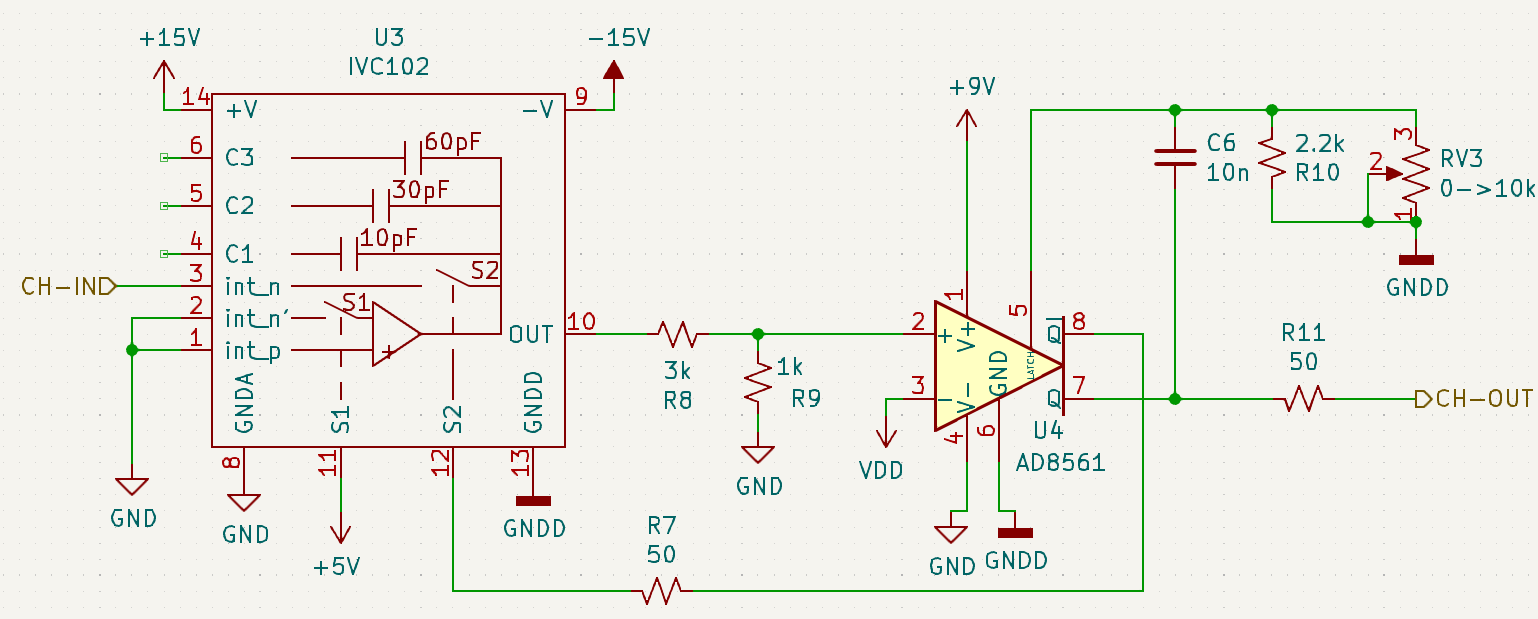
\includegraphics[width=\textwidth]{images/saq_integrator_circuit.png}
\caption{
A schematic of the front-end CSA and trigger components.
The IVC~\citep{ivc_datasheet} chip was chosen as the off-the-shelf integrator for this experiment due to its low input bias current $\ll 750~\unit{fA}$ and variable capacitance.
A voltage divider between resistors R8 and R9 reduces the voltage reference to the comparator by a factor of four.
VDD is a configurable voltage which can be tuned per channel.
}
\label{fig:saq_circuit_kicad}
\end{figure}

\begin{figure}[]
\centering
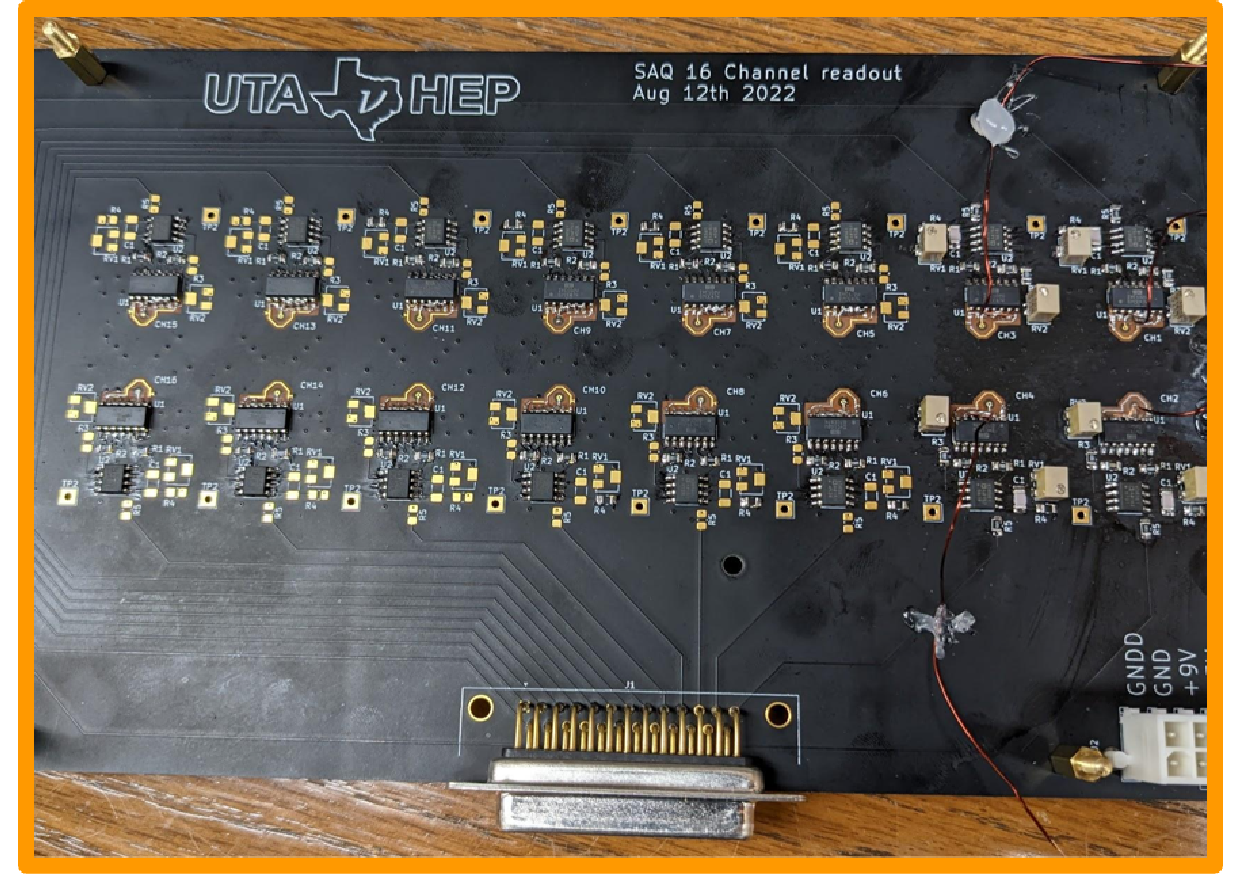
\includegraphics[width=0.7\textwidth]{images/SAQ_16_ivc_readout_board.pdf}
\caption{The SAQ front-end board of 16 input IVC channels.
Each of the 16 channels are based on Figure~\ref{fig:saq_circuit_kicad}.
}
\label{fig:saq_readout_board}
\end{figure}

A simplified diagram of how charge-integrate-reset behavior of SAQ is shown in Figure~\ref{fig:saq_reconstruction}.
The voltage across the integrator increases are charge is accumulated.
Once a specific charge ($Q_{o}$) as accumulated on the integrator, the comparator sends an output pulse that causes a reset and is recorded by digital back-end.
The specific value of charge per channel must be calibrated~(Section~\ref{sec:saq_calib}).
Once the reset stops, charge accumulates until the next reset pulse.

\begin{figure}[]
\centering
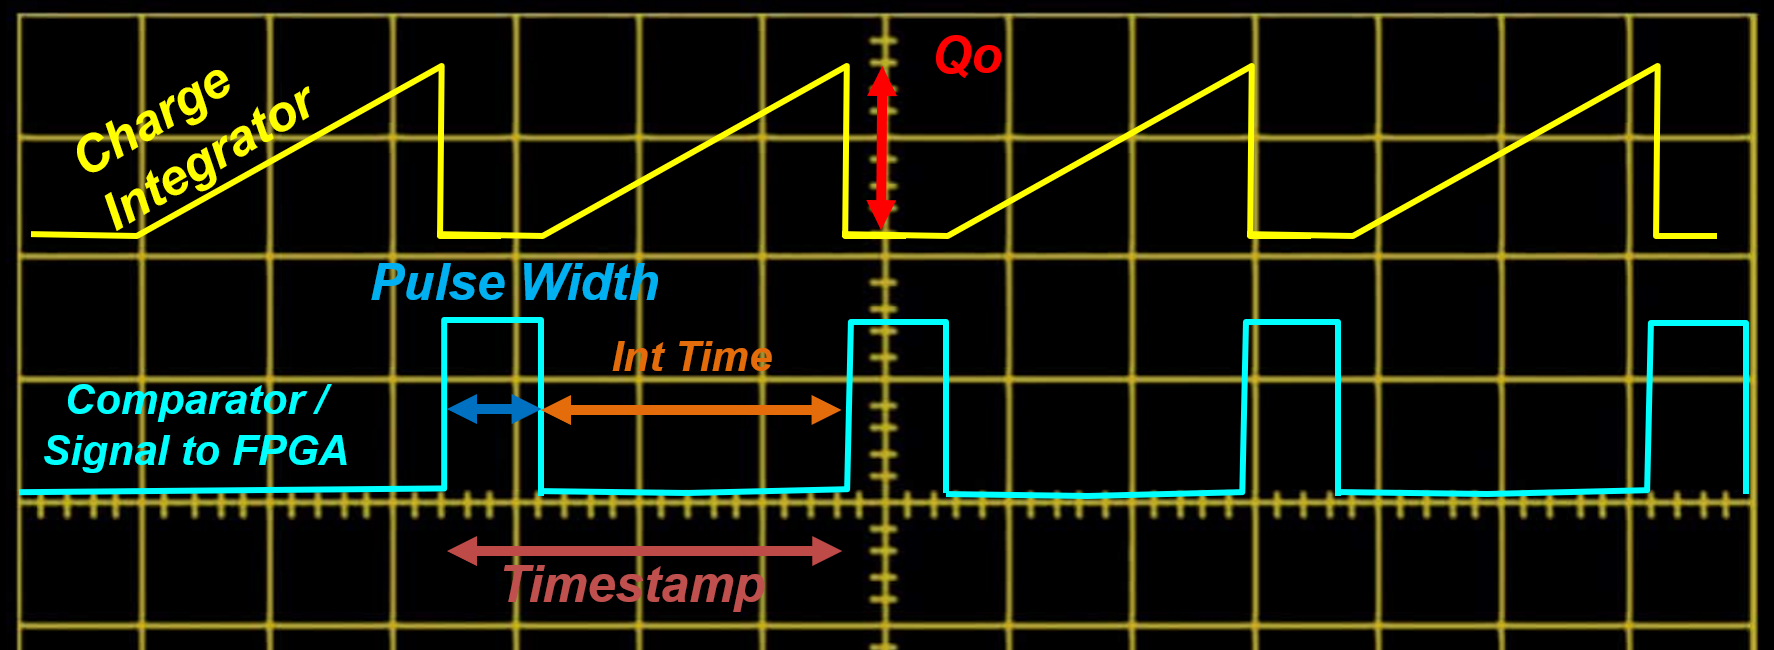
\includegraphics[width=\textwidth]{images/saq_example_reconstruction.png}
\caption{Diagram of voltage waveforms of the integrator (top, yellow) and output (bottom, blue) are shown.
Charge accumulates on the integrator until a value, $Q_{o}$, is reached which causes an output pulse to be sent by the comparator.
During the reset, no charge is accumulated on the integrator so the voltage does not change.
After the reset completes, charge can build back up on the integrator until another reset.
A Reset-Time-Difference (RTD) is the calculated time difference between two timestamp measurements, and includes the time of the pulse-width as well as the true integration time.
}
\label{fig:saq_reconstruction}
\end{figure}

An example of the charge-integrate-reset procedure of the integrator circuit is shown in Figure~\ref{fig:saq_resets}.
Each reset corresponds to a charge accumulation of $\approx 10~\unit{pC}$.
The time difference between each reset shown is equivalent to the amount current accumulated at the IVC~(Equation~\ref{eq:irecon}).
The initial reset occurs $\approx 30~\unit{\mu s}$ after the flash lamp is triggered, which corresponds to the drift speed of electrons in gas, plus the flash lamp response measurement.
The additional resets which occur much latter ($\simeq 100~\unit{\mu s}$) are from currently unknown sources, and are likely either discharges from the GEM or electronic cross-talk.

\begin{figure}[]
\centering
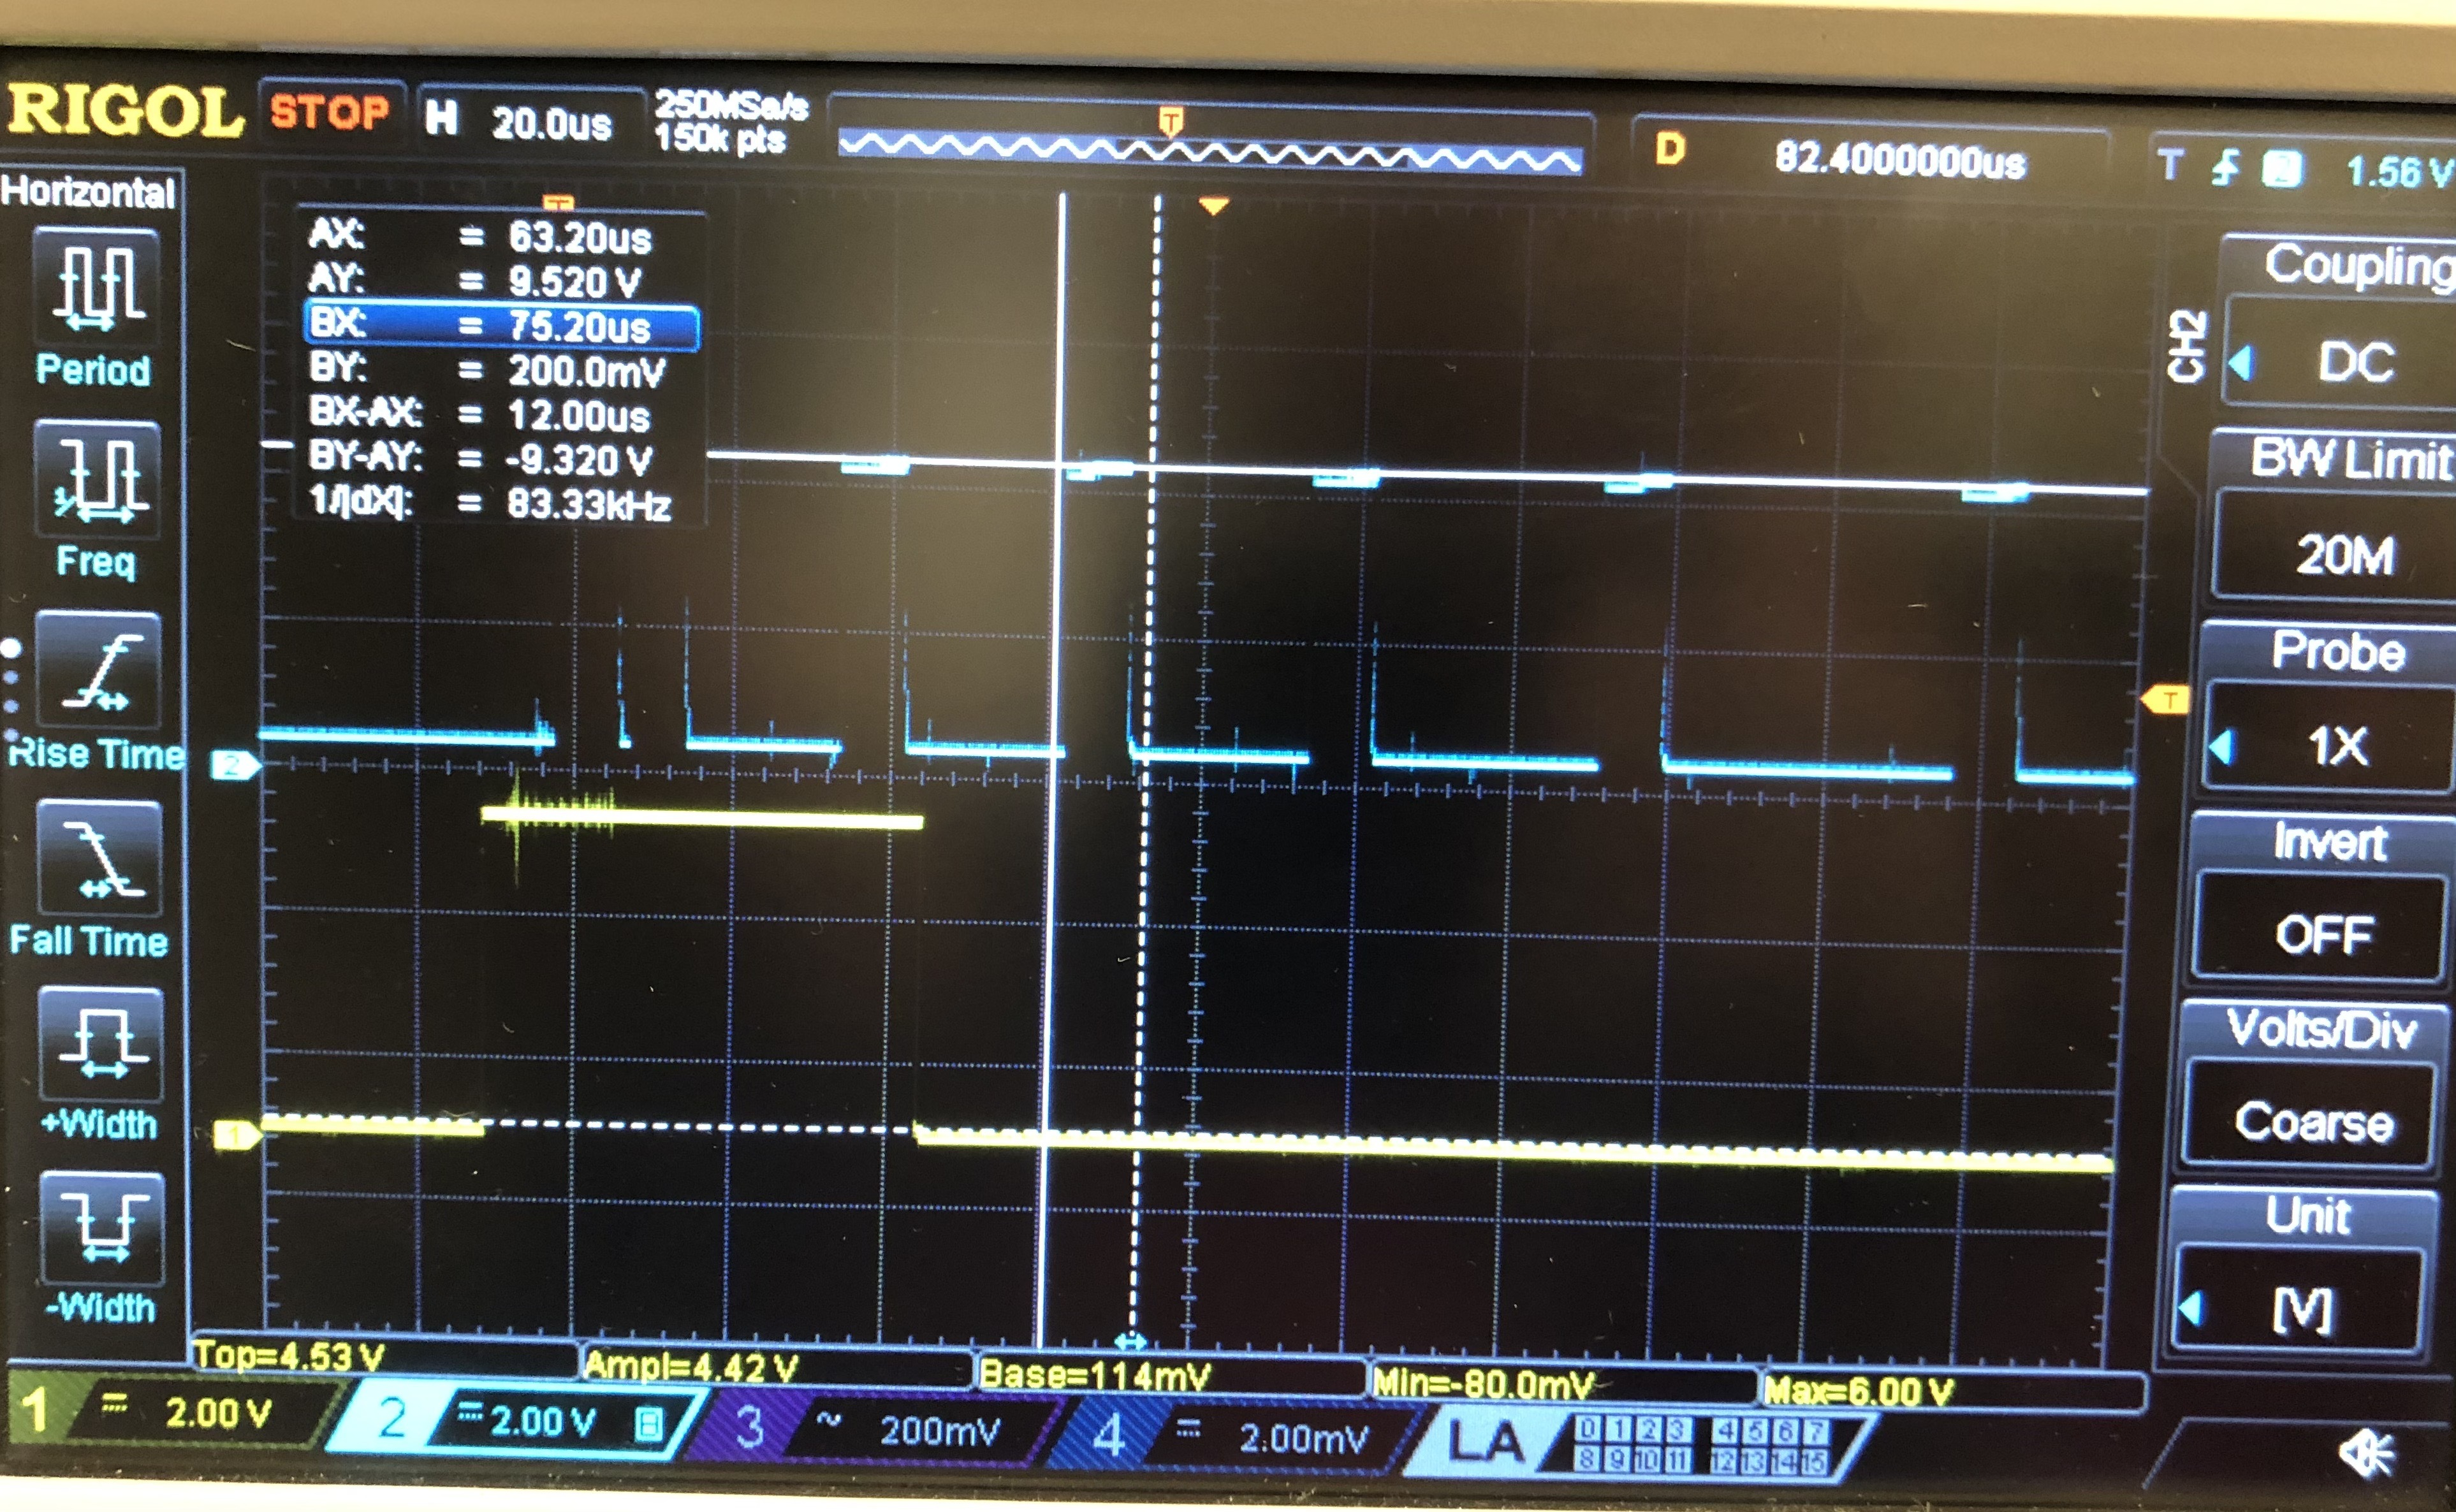
\includegraphics[width=\textwidth]{images/saq_reset_pulse_gem_thickBoard.jpg}
\caption{Waveform measurements of the trigger sent to the Xenon Flash lamp (yellow, bottom), and the reset pulse responses sent by the comparator.
Each reset corresponds to a build up of $\approx 10~\unit{pC}$ of charge stored up on the IVC capacitor.
Seen in the waveform is a decaying amount of charge buildup on the capacitor, which is reflected in the increasing time separation between successive resets.
}
\label{fig:saq_resets}
\end{figure}

\section{Data Acquisition}
All resets are recorded via a Zybo-Z7-20 Digilent FPGA prototype board, which uses an Zynq-7000 System on Chip (SoC).
The clock (30.3~\unit{MHz}) is provided by the Processing System (PS), an ARM Cortex-A9, to the Programmable Logic (PL) in the FPGA.
The PL records a 32-bit counter (the timestamp) on the next clock cycle after the reset, connected as a latch to a single pin input, is driven high.
The reference manual for the Zybo Z7 board used in SAQ can be found at~\citep{zybo_zy_reference}.

The timestamp data and the channel mask are accumulated in a First-In-First-Out (FIFO) buffer.
If any one (or more) of the 16 input channels transitions from low to high and the FIFO register is enabled, data are written to the FIFO.
The input from all 16 channels are recorded at the time of the trigger, regardless of which channel caused the trigger.
Multiple triggers from the same reset pulse are prevented by detecting the rising edge of the reset pulse.
Therefore, in order for a new reset to be recorded on the same channel the reset pulse must first be driven low for at least one clock cycle ($\gtrsim$ 33~\unit{ns}) to reset the latch at the input channel.
This timestamp trigger procedure is identical to the implementation of the Q-Pix digital ASIC presented in Chapter~\ref{chap:qdb}.

A flow chart of the control system for the Zybo is shown in Figure~\ref{fig:saq_diagram}.
The PS connects to both a User-Datagram-Protocol (UDP) and Transmission Control Protocol (TCP) socket on a controlling computer.
The UDP socket on the computer is only a listening socket and receives the timestamp data from the Zybo.
The TCP socket is used to read and write to the control registers on the PL.
Relevant control registers include channel masking, timestamp division, and a write enable to the FIFO.

\begin{figure}[]
\centering
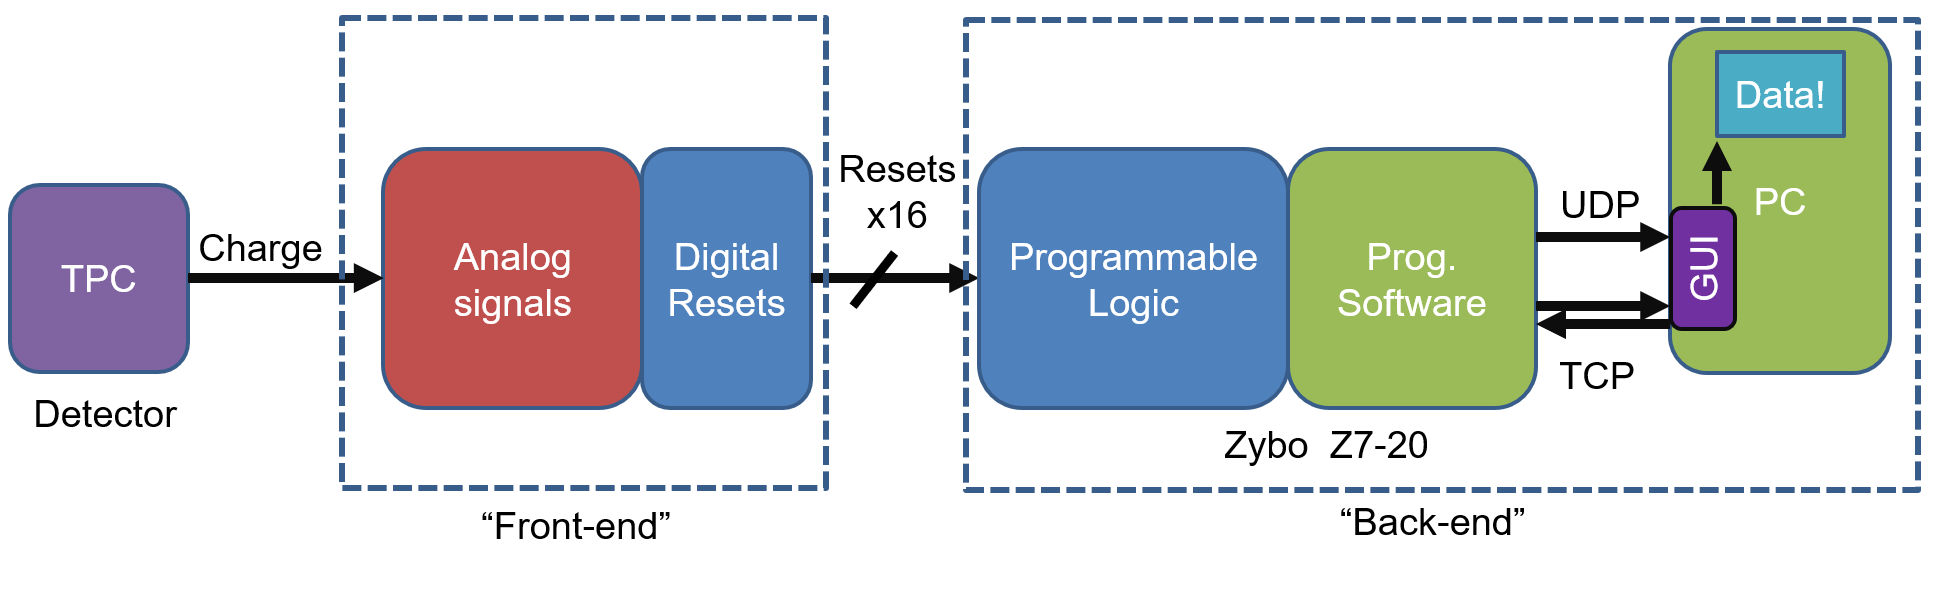
\includegraphics[width=\textwidth]{images/saq_daq_back-end_summary.png}
\caption{SAQ system over view connecting the front-end and back-end parts of a Q-Pix readout.
Gaseous Argon is used for the drift medium of the TPCs at both UTA and Wellesley.
Accumulated charge is read by the front-end which consists of 16 integrating amplifiers each connected to a comparator used as a trigger~\ref{fig:saq_circuit_kicad}.
The back-end board is a Digilent Zybo-Z7-20~(Figure~\ref{fig:saq_zybo}).
}
\label{fig:saq_diagram}
\end{figure}

A summary of the connection ports to the Zybo are shown in Figure~\ref{fig:saq_zybo}.
The Zybo is connected to a desktop computer (PC) via a 1~\unit{GB/s} Ethernet link.
The SAQ timestamp connections use two right-angle connectors.
Also shown in the Figure is the connection to the Q-Pix Digital Board (QDB) presented in Chapter~\ref{chap:qdb}.
Reference 10~\unit{\mu s} pulses at varied frequencies (2-256~\unit{Hz}) are generated in the last marked connector.

\begin{figure}[]
\centering
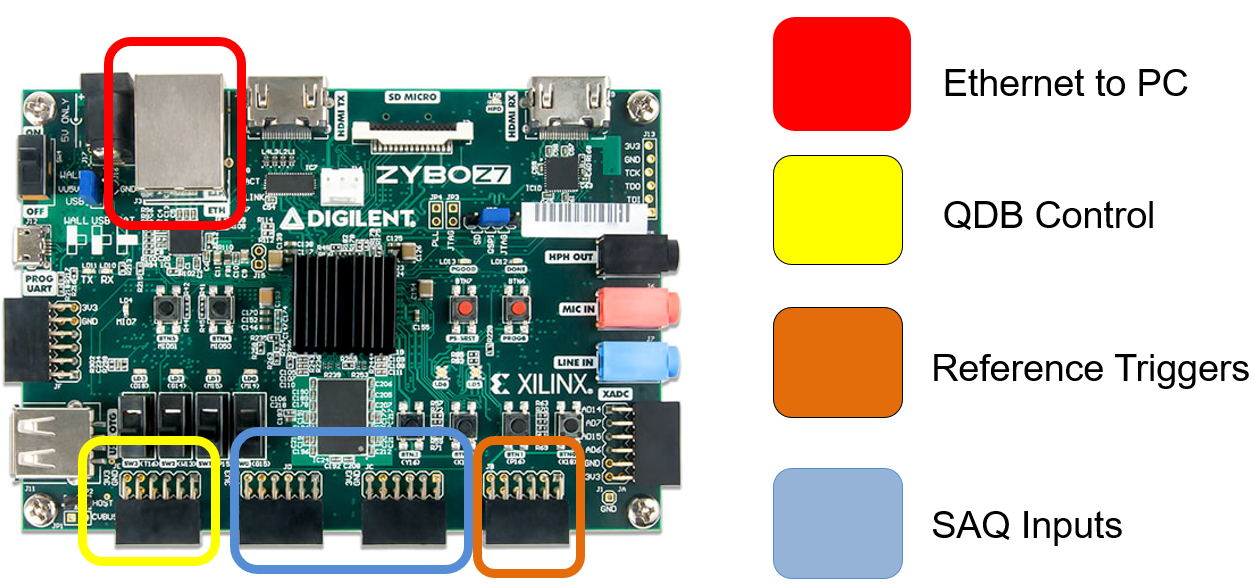
\includegraphics[width=\textwidth]{images/saq_zybo_io_summary.png}
\caption{An image of the data acquisition board from Digilent, Zybo Z7-20. 
This board was chosen for its multiple configurable input channels, as well as the Zynq-based architecture of the onboard FPGA.
Additionally, the use of the Ethernet provides $1~\unit{GB/s}$ transfer speeds, which is more than sufficient for the application.
Packet data transfer rates have been verified with this readout at stable rates of 10~\unit{kHz}.
This board is also used to control the Q-Pix Digital Boards (QDB), discussed in Chapter~\ref{chap:qdb}.
}
\label{fig:saq_zybo}
\end{figure}

The charge integration period for some channels, especially in tests without the GEM, can take several minutes to produce a single reset, so 30 MHz is not always an appropriate frequency at which to discretize timestamps.
A division register can be used to change the effective frequency, allowing RTDs to be timestamped from 30 MHz down to 7 mHz.
The results presented here use a typical division register value of 200, which corresponds to a timestamp frequency of 150~\unit{kHz}.

A summary of the firmware and embedded software is shown in Figure~\ref{fig:saq_firmware}.
The control of the SAQ Data-Acquisition (DAQ) is handled via a Graphical-User-Interface (GUI) which also handles the UDP and TCP sockets.
The data collected by the DAQ are originally written as binary packets to the PC, but are eventually parsed into output ROOT files for analysis.

The data are sent from the PL to the PS and finally to the PC once a (register controlled) number of timestamps are written to the FIFO.
The AXI-Stream FIFO packages the timestamp and channel data in to a singular packet that is then written to the DDR3 memory in the PS.
The PS receives an interrupt signal from the DMA to notify that is received a new packet of data.
The PS then sends all timestamp and channel mask data as a single packet via UDP.
Additional bytes are appended to the packet which include the number of timestamps included in the packet as well as a packet identification number.
The controlling software uses the identification number to flag for any missed packets to notify the user of possible missing data.

\begin{figure}[]
\centering
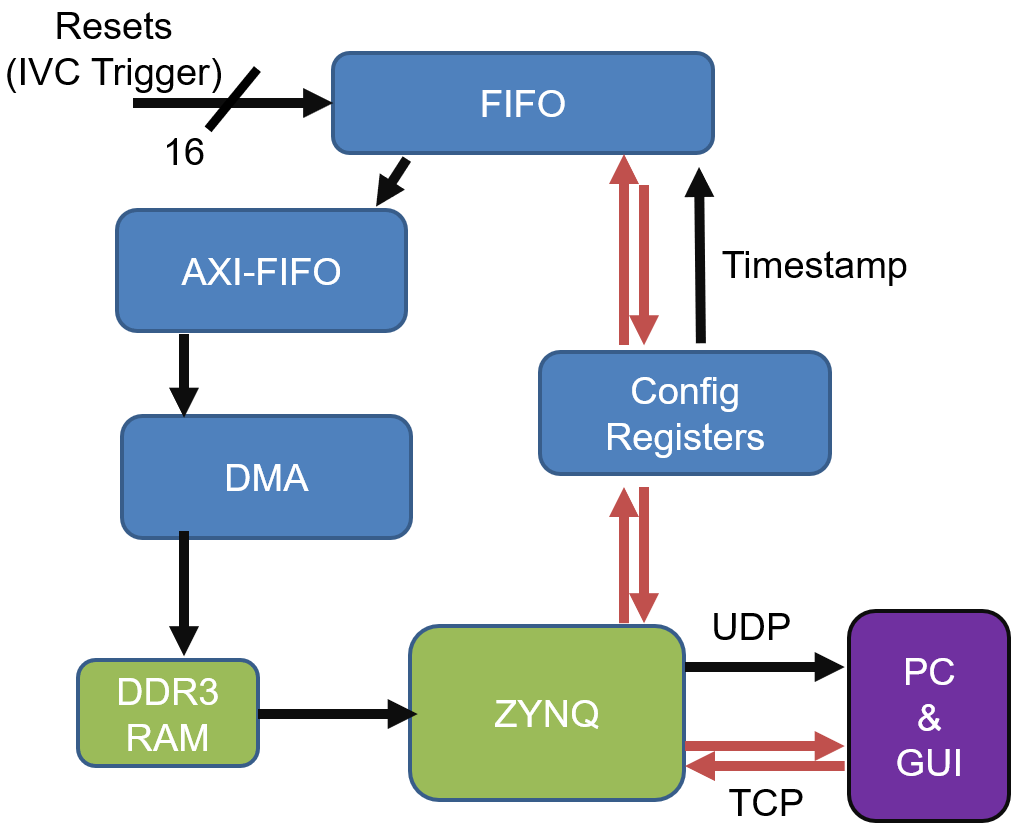
\includegraphics[width=0.5\textwidth]{images/saq_daq_firmware_summary.png}
\caption{A flowchart of the firmware (top, blue), and the embedded software (bottom, green), within the Z-7000 SoC.
A FIFO is used to collect the timestamp and channel mask output from the SAQ Board~\ref{fig:saq_readout_board}.
The AXI-FIFO and Direct-Memory-Access (DMA) send data from the FIFO once a (register controlled) number of timestamps have been written to the FIFO.
These data are collected by the PS and sent via UDP to the PC.
The control registers are configured via TCP within the same GUI~(Figure~\ref{fig:saq_gui}) application that collects and provides real-time plotting of the timestamp data.
}
\label{fig:saq_firmware}
\end{figure}

\begin{figure}[]
\centering
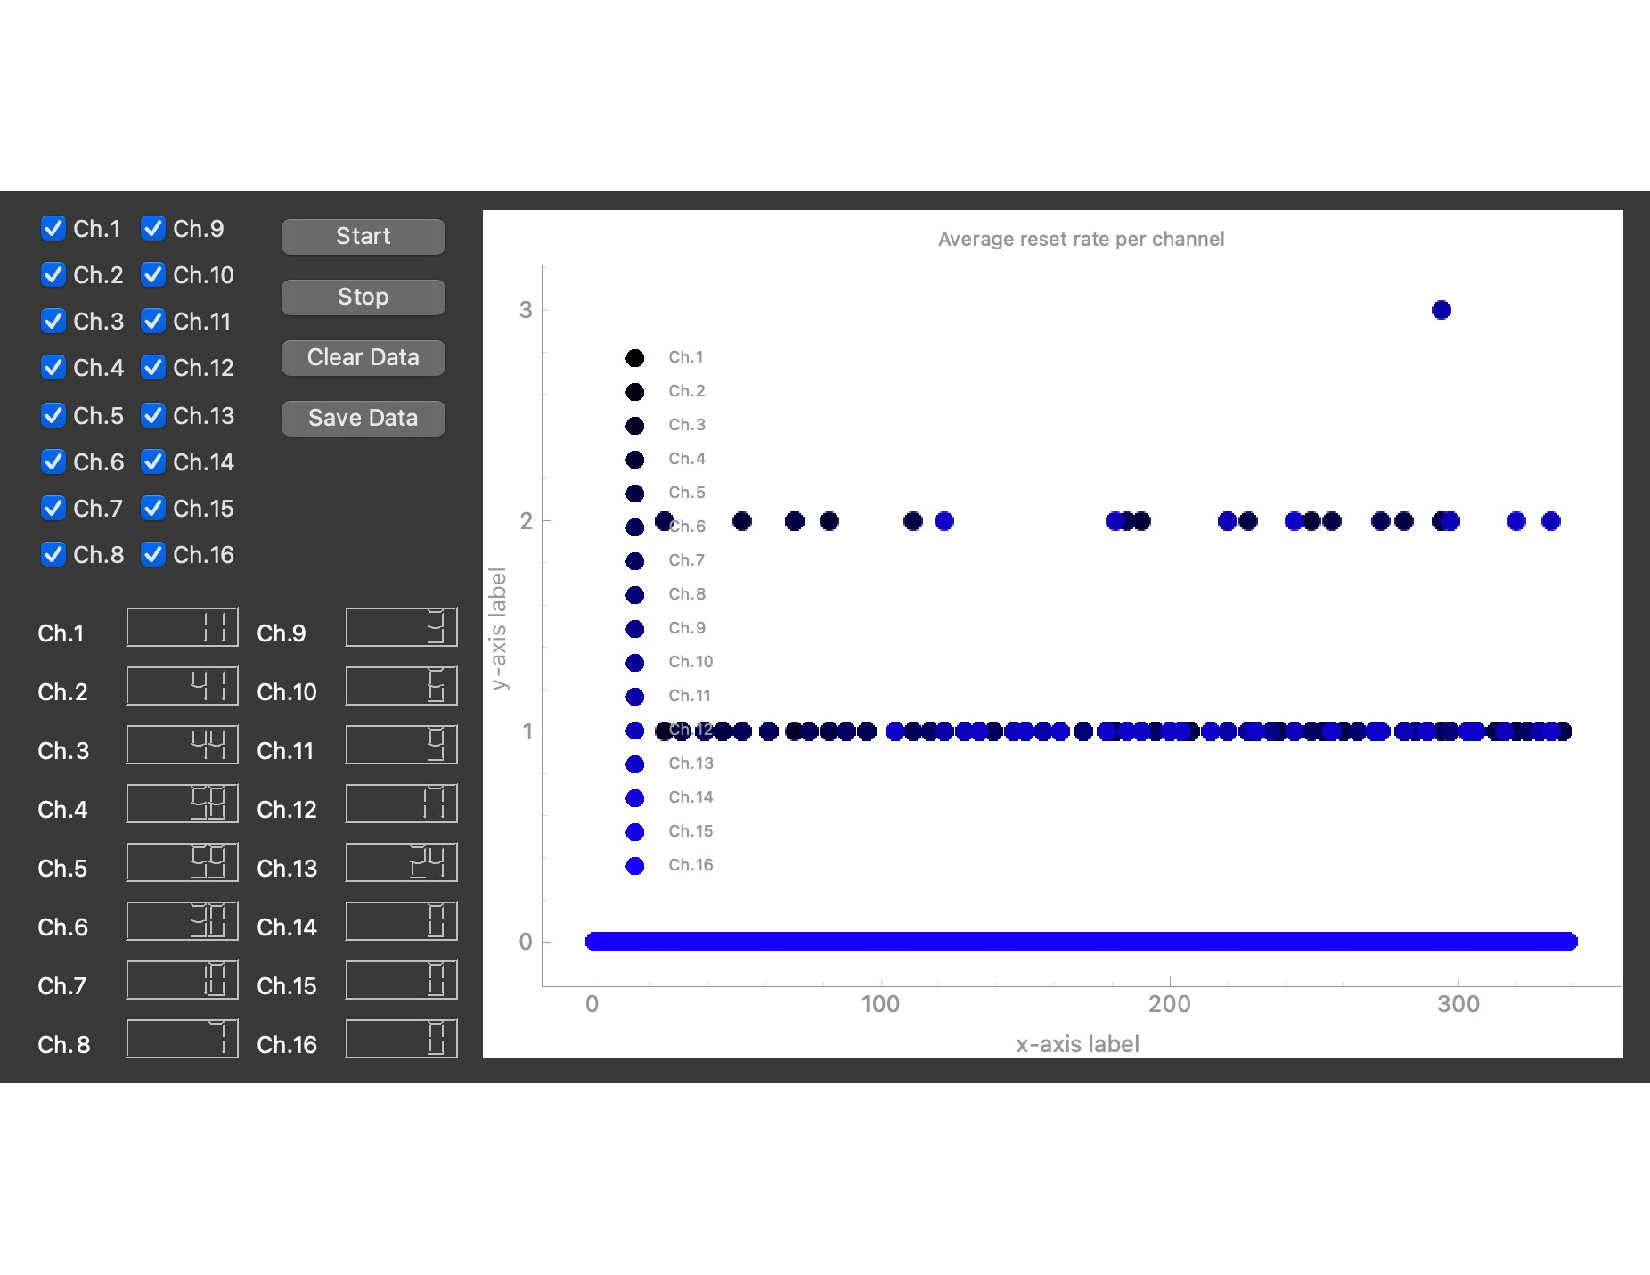
\includegraphics[width=0.9\textwidth]{images/SAQ_gui_resets.pdf}
\caption{The SAQ GUI with real time plotting of incoming resets to the Zybo board.
Every second the GUI updates the number of resets acquired by each of the channels in the previous second.
The GUI allows channel masking features of individual channels shown by the checked boxes in the top left.
}
\label{fig:saq_gui}
\end{figure}

\section{Status and Calibration Procedures}
\label{sec:saq_calib}
The Q-Pix readout is dependent on two factors~(Equation~~\ref{eq:irecon_freq}): the charge and frequency calibrations.
The frequency calibration depends on the stability of the local oscillator and its reliability to accurately record the time of reset.
A drifting local oscillator on the digital board, the Zybo for SAQ, will cause poor reconstructions of current.

A clock calibration is performed by using a reference clock to provide input to the test clock.
The test for the stability of the Zybo is performed with a fixed trigger (10~\unit{kHz}) into the Zybo.
The pulse frequency of 10~\unit{kHz} is chosen so that the pulse width is identical to that produced by the IVC chip~(Section~\ref{sec:saq_integrator}).
The reconstructed timestamp difference gives the period of the input trigger.
Figure~\ref{eq:frequency_reconstruction} shows the Zybo measurements in response to a 10~\unit{kHZ} function generator with 1~\unit{ppm}.

\begin{figure}[]
\centering
\begin{subfigure}{.5\textwidth}
  \centering
  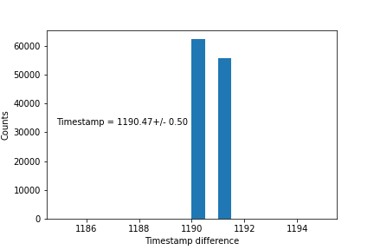
\includegraphics[width=\textwidth]{images/zybo_10khz_timestamp_frequency_calibration.png}
  \caption{}
\end{subfigure}%
\begin{subfigure}{.5\textwidth}
  \centering
  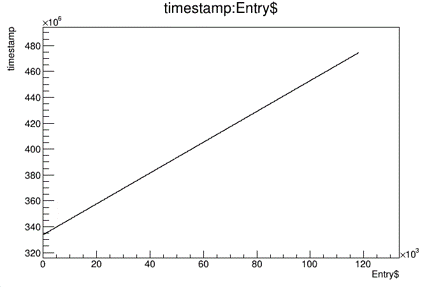
\includegraphics[width=\textwidth]{images/zybo_10khz_timestamp_graph.png}
  \caption{}
\end{subfigure}
\caption{Image of calculated RTDs (left) between successive triggers to the Zybo and the running plot of the timestamp value measured (right).
The clock period on the Zybo was reconstructed to within a single clock cycle, as shown on the left image.
The period of a 10~\unit{kHz} signal is 100~\unit{\mu s} and does not result in an even distribution of clocks, which is why two peaks are shown.
The expected RTD will come no faster than 90~\unit{Hz}, which is more than two orders of magnitude slower than tested here.
}
\label{fig:frequency_reconstructio}
\end{figure}

The effective charge calibration per pixel uses a constant current source as an input to each channel.
A current source is used to deposit a known quantity of charge, which is related to the number of resets by:
\begin{equation}
 \Delta Q = I_{o}t = N_{\mathrm{resets}}Q_{o}
\end{equation}
Where $Q_{o}$ is average charge per reset, $I_{o}$ is the input current from the source current, and $N_{\mathrm{reset}}$ is the number of resets observed in time t.
Then, the charge calibration is:
\begin{equation}~\label{eq:saq_pixel_calib}
 Q_{o} = \frac{I_{o}t}{N_{\mathrm{reset}}}
\end{equation}
Equation~\ref{eq:saq_pixel_calib} is accurate in the limit that the time difference between successive resets is large compared to the pulse-width.
Charge is not accumulated for 10~\unit{\mu s} after every reset, so if the distance between resets during calibration is $\approx$ 1~\unit{s}, the amount of charge lost during the reset is $\frac{\delta Q_{o}}{Q_{o}} \simeq 10^{-5}$.

The Leakage current is measured using a Keithley-6485~\citep{picoammeter-6485-datasheet} pico-ammeter and a nominal estimation of the leakage in the presence of only field and gas measured to be $\approx 0.9~\unit{pA}$ per channel.
Leakage current arises due to non-ideal behavior of the integrator operational amplifier, where the voltage across the two input terminals is nonzero.
The voltage difference causes a continual build-up (or removal of) electronics from the capacitor in the integrating circuit.
Since each reset requires $\approx 10~\unit{pC}$ of charge, the leakage removes roughly one reset from a pixel every 11 seconds.
Therefore, any charge introduced by drift in the TPC to trigger a reset should deposit charge more quickly than 11 seconds to ensure minimal charge loss from leakage.

\subsection{Current Results}
Two different collection plane geometries are tested.
The two different geometries change the amount of exposed copper and are shown in Figure~\ref{fig:trace_boards}.
The "thin" trace (right image) board exposes 6~\unit{mm} wide copper rings around the center of the TPC.
The "thick" trace board inverts the solder mask and exposed copper and instead separates the collection rings by 6~\unit{mm} wide solder mask traces.

\begin{figure}[]
\centering
\begin{subfigure}{.45\textwidth}
  \centering
  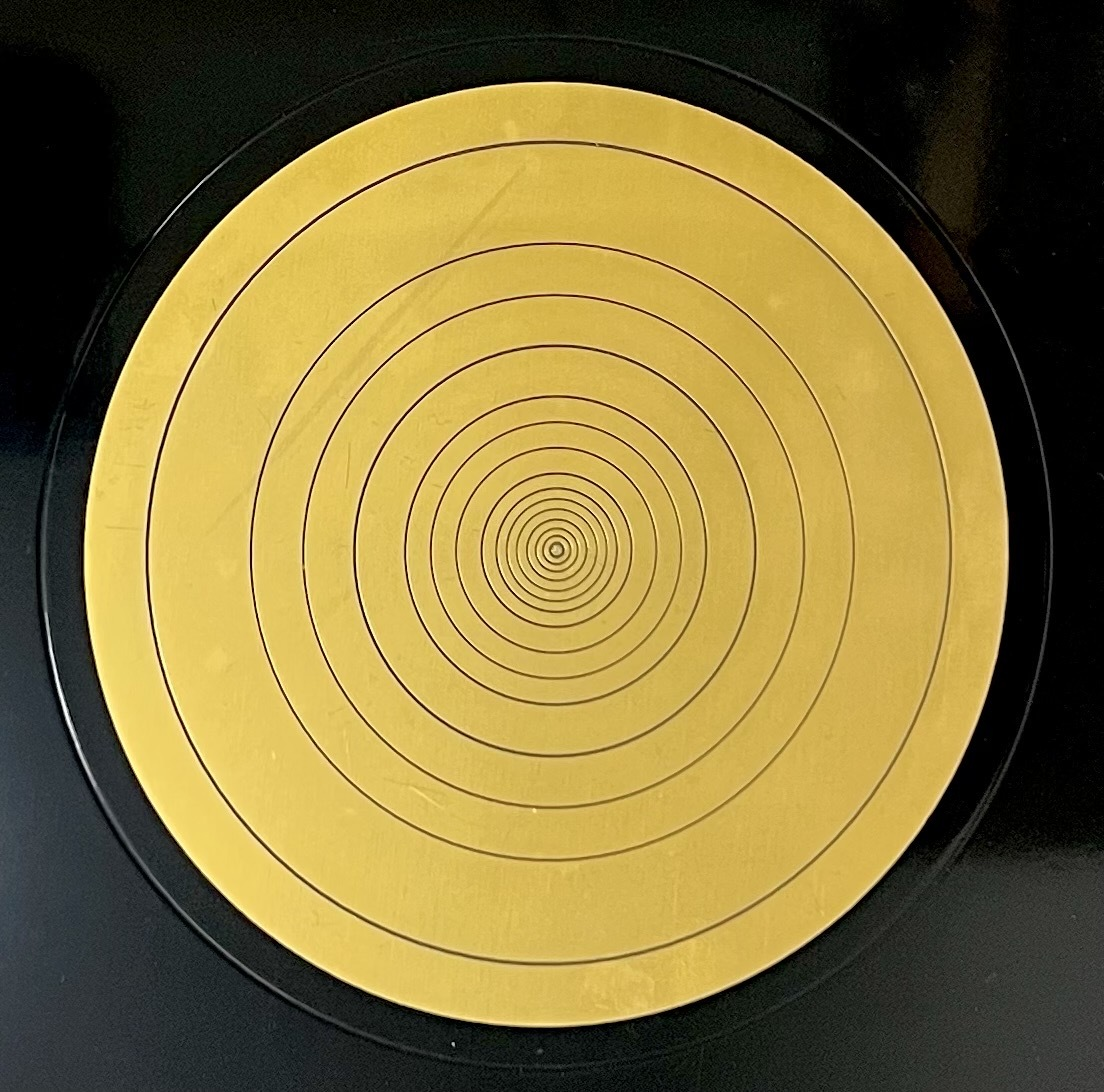
\includegraphics[width=\textwidth]{images/thick_board_example.jpg}
  \caption{}
\end{subfigure}%
\begin{subfigure}{.45\textwidth}
  \centering
  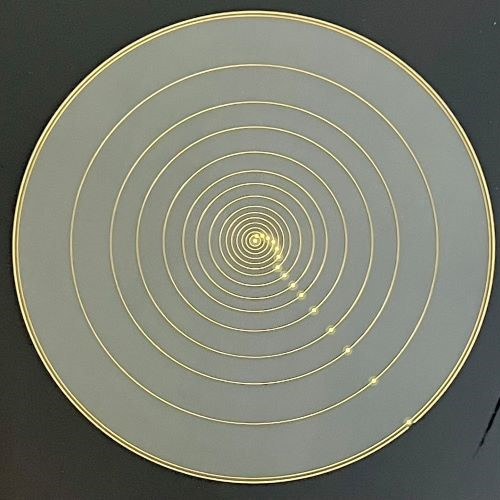
\includegraphics[width=\textwidth]{images/thin_trace_board_example.jpg}
  \caption{}
\end{subfigure}
\caption{Different Trace Boards used in the SAQ Experiment.
The thick trace board (left) differs from the thin trace board (right) in that most of surface area is exposed copper target for the drift electrons.
The thin (right) trace board replaces the collection rings with solder mask, and the solder mask with collection rings.
Because the traces are so small, vias are used to connect the thin collection rings to the input of the integrator channels.
}
\label{fig:trace_boards}
\end{figure}

Examples of data taken with the two collection boards at UTA are shown in Figure~\ref{fig:trace_boards_current_data}.
These data represent multiple five minute charge collection runs using the thick and thin trace boards.
One of the current uncertainties is the large difference for the outer channel.

\begin{figure}[]
\centering
\begin{subfigure}{.45\textwidth}
  \centering
  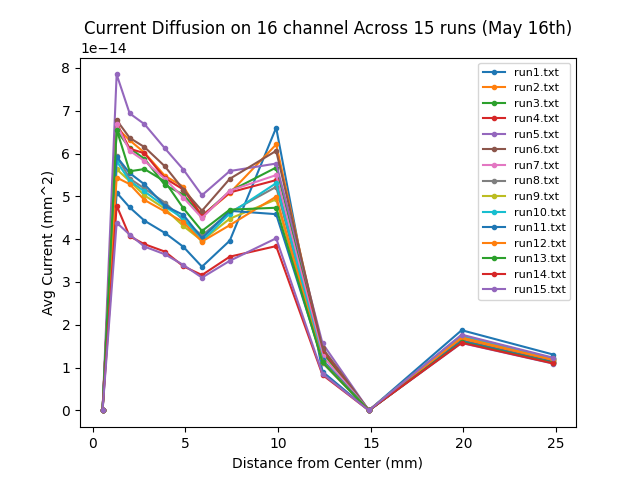
\includegraphics[width=\textwidth]{images/fullBoard_ConvertedAvgCurrentDiffusion.png}
  \caption{}
\end{subfigure}%
\begin{subfigure}{.45\textwidth}
  \centering
  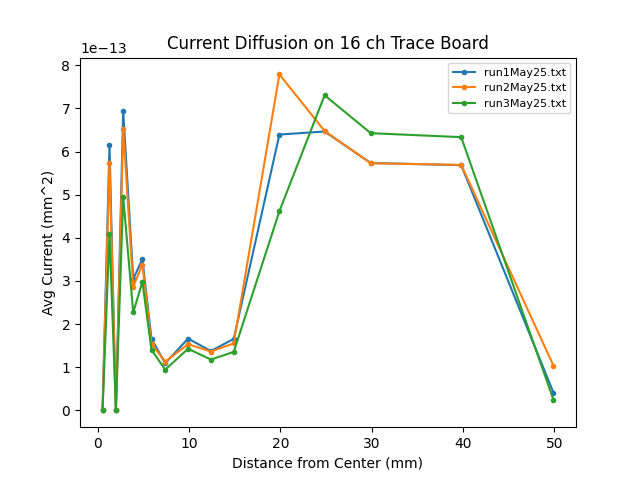
\includegraphics[width=\textwidth]{images/traceBoard_ConvertedAvgCurrentDiffusion.png}
  \caption{}
\end{subfigure}
\caption{Different Trace Boards used in the SAQ Experiment.
The thick trace board (left) differs from the thin trace board (right) in that most of the surface area in the field cage can collect electrons.
The thin (right) trace board replaces the collection rings with solder mask, and the solder mask with collection rings.
Because the traces are so small, vias are used to connect the thin collection rings to the input of the integrator.
}
\label{fig:trace_boards_current_data}
\end{figure}

A plot of initial results from the WC group are shown in Figure~\ref{fig:saq_first_diffusion_measurement}.
These data represent an averaged number of resets divided by the area of the ring on the collection board.
These data indicate that center channels acquire more charge (produce more resets) than outer channels.

\begin{figure}[t!]
\centering
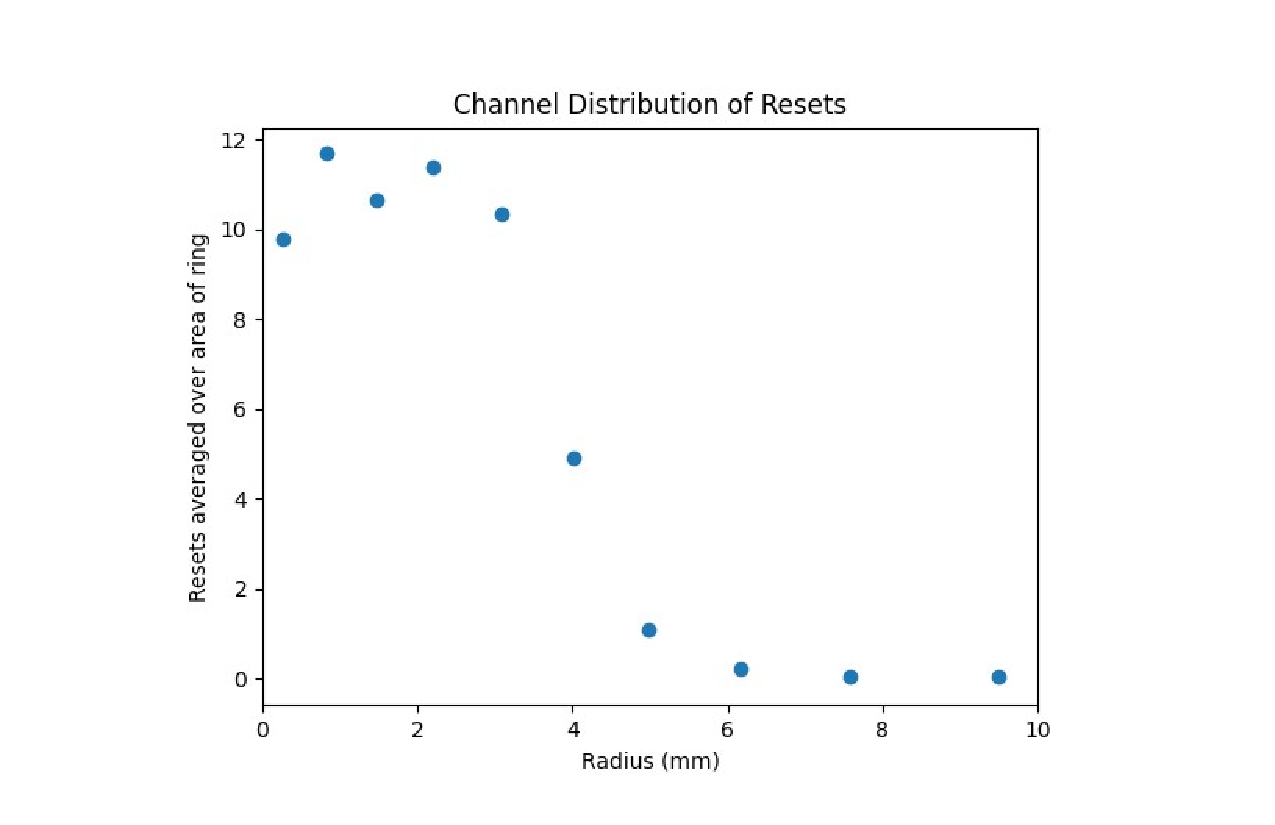
\includegraphics[width=0.95\textwidth]{images/SAQ_first_diffusion_measurement.pdf}
\caption{First diffusion measurement in P-10 gas performed at Wellesley University.
The "double peak" feature is thought to be due to an off-center electron source.
Analysis is currently underway to characterize how charge collection would vary from an offset electron center.
}
\label{fig:saq_first_diffusion_measurement}
\end{figure}

\section{Summary and Future Tests}
Although the diffusion measurements of SAQ are not complete at the time of the writing of this thesis, the work contributed by the author has been demonstrated.
Timestamp data for various gas based TPCs have been collected and been shown to result from accumulated charge on an integrating circuit.
These first tests demonstrate the Q-Pix front-end capability with off-the-shelf components.
The work that remains for SAQ is a characterization of the TPC, GEM, and electric fields, not the front-end readout technology, which is the aim of this thesis.

Work still remains to understand charge accumulation data presented at UTA~(Figure~\ref{fig:trace_boards_current_data}) and WC~(Figure~\ref{fig:saq_first_diffusion_measurement}).
Simulations are being performed to understand the differences between the electric fields with the two different charge collection boards.
Additional tests are underway to understand the behavior of the GEM, and to deduce the charge source causing the delayed resets in some channels, as seen in Figure~\ref{fig:saq_resets}.
